%--------------------------------------------------------------------------------- PACKAGES AND OTHER DOCUMENT CONFIGURATIONS
%---------------------------------------------------------------------------------

\documentclass[
11pt, % The default document font size, options: 10pt, 11pt, 12pt
oneside, % alternatives: oneside, twoside
british, % alternatives: easy, medium, hard
doublespacing, % alternatives: singlespacing, onehalfspacing or doublespacing
headsepline,
]{MastersDoctoralThesis} % The class file specifying the document structure

\usepackage[utf8]{inputenc} % Required for inputting international characters
\usepackage[T1]{fontenc} % Output font encoding for international characters
\usepackage{mathpazo} % Use the Palatino font by default
\usepackage[autostyle=true]{csquotes} % Required to generate language-dependent quotes in the bibliography
\usepackage{amssymb}
\usepackage{enumitem} 
\usepackage{listings}
\usepackage{graphicx}
\usepackage{xspace}
\usepackage[export]{adjustbox}
\usepackage{xcolor}
\usepackage[font={small}]{caption}
\usepackage{supertabular}
\usepackage{float}
\usepackage{amsmath}
\usepackage{svg}
\usepackage{courier} %% Sets font for listing as Courier.
\usepackage{listings, xcolor}
\usepackage{booktabs}
\usepackage{tabularx}
\usepackage{makecell} 
\usepackage{multirow}
\usepackage[backend=biber,style=numeric,citestyle=numeric,sorting=none,natbib=true]{biblatex}


  

\usepackage{ifthen}


\newcommand{\secref}[1]{Section~\ref{#1}\xspace}
\newcommand{\capref}[1]{\textit{Chapter~\ref{#1}\xspace}}
\newcommand{\figref}[1]{Fig.~\ref{#1}\xspace}
\newcommand{\listref}[1]{Listing~\ref{#1}\xspace}
\newcommand{\tabref}[1]{Table~\ref{#1}\xspace}

\newcommand{\etc}{etc.\xspace}
\newcommand{\ie}{\emph{i.e.,}\xspace}
\newcommand{\eg}{\emph{e.g.,}\xspace}
\newcommand{\etal}{\emph{et~al.}\xspace}

\newcommand{\RQ}[1]{RQ$_{\textbf{#1}}$\xspace}


\colorlet{punct}{red!60!black}
\definecolor{background}{HTML}{EEEEEE}
\definecolor{delim}{RGB}{20,105,176}
\colorlet{numb}{magenta!60!black}





\lstset{
tabsize = 4, %% set tab space width
showstringspaces = false, %% prevent space marking in strings, string is defined as the text that is generally printed directly to the console
numbers = left, %% display line numbers on the left
commentstyle = \color{green}, %% set comment color
keywordstyle = \color{blue}, %% set keyword color
stringstyle = \color{red}, %% set string color
rulecolor = \color{black}, %% set frame color to avoid being affected by text color
basicstyle = \small \ttfamily , %% set listing font and size
breaklines = true, %% enable line breaking
numberstyle = \tiny,
}

\lstdefinelanguage{json}{
    basicstyle=\normalfont\ttfamily,
    numbers=left,
    numberstyle=\scriptsize,
    stepnumber=1,
    numbersep=8pt,
    showstringspaces=false,
    breaklines=true,
    frame=lines,
    backgroundcolor=\color{background},
    literate=
     *{0}{{{\color{numb}0}}}{1}
      {1}{{{\color{numb}1}}}{1}
      {2}{{{\color{numb}2}}}{1}
      {3}{{{\color{numb}3}}}{1}
      {4}{{{\color{numb}4}}}{1}
      {5}{{{\color{numb}5}}}{1}
      {6}{{{\color{numb}6}}}{1}
      {7}{{{\color{numb}7}}}{1}
      {8}{{{\color{numb}8}}}{1}
      {9}{{{\color{numb}9}}}{1}
      {:}{{{\color{punct}{:}}}}{1}
      {,}{{{\color{punct}{,}}}}{1}
      {\{}{{{\color{delim}{\{}}}}{1}
      {\}}{{{\color{delim}{\}}}}}{1}
      {[}{{{\color{delim}{[}}}}{1}
      {]}{{{\color{delim}{]}}}}{1},
}



\def\BibTeX{{\rm B\kern-.05em{\sc i\kern-.025em b}\kern-.08em
    T\kern-.1667em\lower.7ex\hbox{E}\kern-.125emX}}

\addbibresource{ref.bib} % The filename of the bibliography


%---------------------------------------------------------------------------------
%	MARGIN SETTINGS
%---------------------------------------------------------------------------------
\geometry{
	paper=a4paper, % Change to letterpaper for US letter
	inner=2.5cm, % Inner margin
	outer=3.8cm, % Outer margin
	bindingoffset=.5cm, % Binding offset
	top=1.5cm, % Top margin
	bottom=1.5cm, % Bottom margin
	%showframe, % Uncomment to show how the type block is set on the page
}

%---------------------------------------------------------------------------------
%	THESIS INFORMATION
%---------------------------------------------------------------------------------
\thesistitle{An Empirical Exploration of Deep Learning Techniques for Automated Enhancement of Code Readability in Large-Scale Software Repositories} % Your thesis title, this is used in the title and abstract, print it elsewhere with \ttitle
\supervisor{Prof. Simone \textsc{Scalabrino} \\[5ex] Dr. Antonio \textsc{Vitale} } % Your supervisor's name, this is used in the title page, print it elsewhere with \supname
\degree{Computer Science} % Your degree name, this is used in the title page and abstract, print it elsewhere with \degreename
\author{Marco \textsc{Omicini}} % Your name, this is used in the title page and abstract, print it elsewhere with \authorname

% Your subject area, print it elsewhere with \subjectname
\subject{Automated Software Delivery} 
% Your university's name and URL, this is used in the title page and abstract, print it elsewhere with \univname
\university{\href{https://www.unimol.it/}{UNIVERSITY OF MOLISE}} 
% Your department's name and URL, this is used in the title page and abstract, print it elsewhere with \deptname
\department{\href{http://dipbioter.unimol.it/}{Department of Biosciences and Territory}} 


\AtBeginDocument{
    \hypersetup{pdftitle=\ttitle} % Set the PDF's title to your title
    \hypersetup{pdfauthor=\authorname} % Set the PDF's author to your name
}



\begin{document}
\renewenvironment{abstract}

\frontmatter % Use roman page numbering style (i, ii, iii, iv...) for the pre-content pages

\pagestyle{plain} % Default to the plain heading style until the thesis style is called for the body content

%---------------------------------------------------------------------------------
%	TITLE PAGE
%---------------------------------------------------------------------------------
\begin{titlepage}
	\begin{center}
		\vspace{.06\textheight}
		{\scshape\LARGE \univname\par}\vspace{0.5cm} % University name
		{\scshape\large \deptname\par}\vspace{1cm} % University name
		
\includegraphics[width=0.25\textwidth]{figs/logo} % University/department logo
		\vspace{1cm}

		\textsc{\Large Bachelor's Thesis in \degreename}\\[0.5cm] % Thesis type

		\HRule \\[0.2cm] % Horizontal line
		{\huge \bfseries \ttitle\par}\vspace{0.2cm} % Thesis title
		\HRule \\[1.5cm] % Horizontal line

		\begin{minipage}[t]{0.4\textwidth}
			\begin{flushleft} \large
				\emph{Author:}\\
				\authorname % Author name - remove the \href bracket to remove the link
			\end{flushleft}
		\end{minipage}
		\begin{minipage}[t]{0.4\textwidth}
			\begin{flushright} \large
				\emph{Supervisor:} \\
				\supname
			\end{flushright}
		\end{minipage}\\[2cm]
		\centerline{\large \subjectname}
		\smallskip
		{\large Academic Year 2022/2023}\\[2cm] % Date
		\vfill
	\end{center}
\end{titlepage}

%---------------------------------------------------------------------------------
%	DEDICATION PAGE
%---------------------------------------------------------------------------------

%%%%%%%%%%%%%%%%%%%%%%%%%%%%%%%%%%%%%%%%%%%%%%%%%%%%%%%%%%%
% Dedica
\vspace{5em}
\begin{flushright}
{\normalsize \textit{Dedico questa tesi a tutti noi,}\\ \textit{cercatori di conoscenza, appassionati di computers}}\\
\end{flushright}

\clearpage{\pagestyle{empty}\cleardoublepage}


%---------------------------------------------------------------------------------
%	ABSTRACT PAGE
%---------------------------------------------------------------------------------
% \pagenumbering{gobble}
% \vspace*{50px}
% \centerline{\textbf{Abstract}}
% \bigskip
% \begin{abstract}
% 	\addchaptertocentry{\abstractname} % Add the abstract to the table of contents
% 	Code readability plays a critical role in software development, especially in an environment where the complexity of information systems continues to evolve. To address this challenge, emerging solutions seek to automate the process of improving code readability, recognizing its critical importance in ensuring maintainability and scalability of software projects. This experimental study aims to investigate the application of the first-of-its-kind deep learning model in the scientific field to enhance the readability of extended code. To tackle such an important undertaking, we adopted a software repository mining approach, followed by a pipeline of operations used to generate our primary dataset. Next, this dataset was analyzed by our selected deep learning model, which proposed a number of modifications aimed at improving the readability of the code. These modifications were then analyzed, revealing that while they contributed in part to slightly improving the readability of the code, they often altered the behavior of the original software suggesting that, although the practice shows promise, there is still ample room for improvement.

% \end{abstract}


%---------------------------------------------------------------------------------
%	LIST OF CONTENTS/FIGURES/TABLES PAGES
%---------------------------------------------------------------------------------
% Begin roman (I, II, III...) page numbering
\newpage\pagenumbering{Roman}

% Prints the main table of contents
\tableofcontents
%---------------------------------------------------------------------------------
%	THESIS CONTENT - CHAPTERS
%---------------------------------------------------------------------------------
% Begin numeric (1,2,3...) page numbering
\mainmatter

% Return the page headers back to the "thesis" style
\pagestyle{thesis}

% Include the chapters of the thesis as separate files from the Chapters folder
\chapter{Introduction}
\label{Chapter1}

\section{Application Context}
In the context of software systems evolution, it is universally recognized that adopting code maintenance practices is essential to mitigate the intrinsic technical debt in software development. This debt encompasses costs that accrue during the development process, such as writing unreadable code, lack of documentation, and the presence of duplicate, unused, or untested elements, all of which inevitably contribute to software degradation over time. Technical debt poses a challenge as it slows down the development process, leading to increased costs for companies. Over time, as Besker \etal \cite{Besker2018} shows the release of new features experiences a slowdown concurrently with the increase in technical debt; As pointed out by Rios \etal \cite{Rios2018} study on technical debt, this can lead to experience financial losses. To counteract this phenomenon and ensure greater software longevity, it is common practice to employ refactoring techniques. Refactoring involves modifying the source code to improve readability, maintainability, and comprehensibility. Unreadable code exhibits various characteristics, including excessively long procedures/classes, redundant or unclear comments, lack of documentation, and the use of so-called "magic numbers," along with the presence of unused code. Refactoring, therefore, plays a fundamental role in software systems evolution, and the automation of this activity represents an active area of research. The goal is to make these refactoring practices automatic since refactoring is a lengthy and meticulous activity, often difficult to execute correctly due to the need to deeply understand the source code. Readability thus emerges as a fundamental yet often overlooked aspect underlying proper refactoring and, consequently, the correct evolution of the software system.

\section{Motivation and Objectives}
Several studies have emphasized the critical role of code readability in software maintenance. While acknowledging the multifaceted and subjective nature of code readability, it is widely accepted that easily understandable code facilitates comprehension, modification, and maintenance. Some research has proposed metrics to evaluate code readability, while others have focused solely on specific aspects of automated readability improvement, such as variable naming. However, only recently a study has been proposed aiming to use machine learning models to holistically improve code readability. This cutting\-edge study has spurred us to undertake this experimental thesis, as it is the first time that there is a proposal to concretely examine the potential of deep learning models in enhancing code readability within extensive projects. Our experimental thesis aims to evaluate the impact of using deep learning models on code readability and, consequently, on the overall software development experience.
With this in mind, we have formulated the following research questions to guide our investigation:


\begin{flushleft}
	\fcolorbox{gray!20}{gray!20}{\begin{varwidth}{\dimexpr\textwidth-2\fboxsep-2\fboxrule\relax}
			$\mathbf{RQ1}$: \emph{What is the impact of applying automatic code readability enhancement considering snippets with varying levels of readability, namely low, medium, and high?}
		\end{varwidth}}
\end{flushleft}
With this question, we aim to understand how the model performs in different contexts (low, medium, high readability) and therefore determine if and especially in which context it excels in improving code readability.

\begin{flushleft}
	\fcolorbox{gray!20}{gray!20}{\begin{varwidth}{\dimexpr\textwidth-2\fboxsep-2\fboxrule\relax}
			$\mathbf{RQ2}$: \emph{Does readability enhancement through deep learning models change code behavior?}
		\end{varwidth}}
\end{flushleft}
Here, we are interested in understanding whether the model, by improving code readability, can alter the behavior of the code itself. This is a critical aspect because any modification to the source code could potentially introduce errors or undesired behaviors, thus mitigating the practice of refactoring inherent in the application of such a model.


\section{Results}
The results indicate that the model is capable of enhancing the readability of poorly readable and moderately readable code snippets, albeit to a limited extent, offering improvements of up to 5\% at most. Regarding highly readable methods, the model does not yield significant enhancements; in fact, in some cases, a decrease in readability is observed.\newline
Except for a specific case study where there is no alteration of correctness, the results demonstrate that the model tends to primarily alter the behavior of code for automatic refactoring of poorly readable methods. In the case of moderately readable methods, it is observed that correctness is preserved in 33\% of cases, while in the remaining 67\%, such correctness is compromised. For highly readable methods, the correctness of procedures is usually preserved.
\section{Thesis Structure and Organization}
The study is structured into 6 phases (divided into chapters), each addressing different topics. In \capref{Chapter2}, we will explore the state-of-the-art literature, aiming to delineate the overall landscape of the problem and the currently available solutions. In \capref{Chapter3}, we will delve into the approach utilized to conduct this experimental study, while \capref{Chapter4} will discuss the case study and the various outcomes obtained. Subsequently, in \capref{Chapter5}, we will discuss the limitations and factors that may have influenced the validity of this study. Finally, in \capref{Chapter6}, we will present the conclusions and acknowledgments.

\chapter{Background and Related Work}
\label{Chapter2}


\section{Code readability}

Code readability stands as a pivotal element in software maintenance, a fact supported by ample evidence in the literature. Tufano et al. \cite{Tufano2015} delineate various factors indicating when code quality deteriorates, commonly referred to as "code smells." The study shows that code smells are often introduced upon file creation or repeated modification of the same file. It is demonstrated that the file creator often introduces them, and this typically occurs months before a deadline or when the developer is under heavy workload. Sedano et al. \cite{Sedano2016} illustrate that developers are often unaware of the difficulty another developer faces in reading the code they produce, and how this awareness eventually drives developers to write more readable code, whether the initial code was readable or not. Scalabrino et al. \cite{Scalabrino2018} propose a model aimed at estimating code readability by improving upon previous state-of-the-art models. These improvements are based on previously unexplored textual features such as Comments and Identifiers consistency, which measures the overlap of terms used in comments with those used in the code body, and Identifier terms in dictionary, a metric aiming to identify how many of the words used belong to the English dictionary, as it has been shown that abbreviated naming is often correlated with lower readability.\newline
Understanding these indicators is crucial, although their effectiveness is questioned by the study conducted by Fakhoury et al. \cite{Fakhoury2019}, demonstrating that these metrics may be partially ineffective in capturing what a developer would define as an improvement in code readability. The study shows that the existing models are unable to capture improvements in readability during software maintenance and proposes additional metrics to enhance their effectiveness. Additionally, Travares et al. \cite{Travares2020} shed light on the intricacy of this issue, cautioning that attempts to enhance code readability through automated refactoring can inadvertently worsen the situation. Indeed, it has been shown that automated refactoring practices may introduce code smells. Another pivotal study conducted by Oliveira et al. \cite{Oliviera2020} exposes some shortcomings in evaluation studies on readability conducted using human subjects, revealing that different approaches require different skills and that only some of these skills are utilized in these evaluations.

\section{Machine learning to improve code readability}

Enhancing code readability using machine learning models represents a dynamic area of research, with several studies showcasing their efficacy in automating refactoring tasks. For instance, Piantadosi \cite{Piantadosi2020} demonstrated how software tends to evolve and lose readability to a relevant extent as features are added and changes are made to it, and outlined guidelines such as small incremental commits and frequent refactoring practices to mitigate this issue. This observation underscores the importance of the study mentioned in the preceding paragraph, which investigates the efficacy of deep learning techniques in enhancing code readability. By addressing this issue, the study contributes to mitigating the potential loss of readability in evolving software systems. \newline
Regarding the automation of refactoring activities, some studies have focused on automatically improving certain characteristics that describe more readable code. The study conducted by Mastropaolo et al. \cite{Mastropaolo2023} demonstrates how deep learning models can be applied to automate variable renaming as a technique to enhance readability. Finally, Vitale et al. \cite{Vitale2023}, the study that profoundly influenced our research direction, significantly advanced the field of automated refactoring. This study introduced a deep learning model capable of suggesting optimal actions (such as renaming, code extraction, styling operations, etc.) to enhance code readability. By training a neural network on a dataset comprising 122k commits, this approach effectively modified code without altering its behavior in 69\% of cases and improved readability in Java code snippets by 79.4\%. These findings served as the foundation for our research, which aimed to apply this model in real-world application contexts.





\chapter{Empirical Study Design}
\label{Chapter3}
In this empirical study, our aim was to evaluate the effectiveness of the-state-of-art deep learning model (referred to as the Code readability enhancement model) proposed by Vitale \etal \cite{Vitale2023} in improving the readability of Java code. To accomplish this, we decided to extract and evaluate the readability of code samples before and after applying the model, utilizing a tool aimed at assessing and measuring the readability of a given piece of code. The objective was to understand if and how this model could enhance readability. Therefore, we extracted a set of Java code snippets and evaluated their readability both before and after applying the model. Our analysis focused on assessing any improvements in readability brought about by the model's interventions.\newline
Our study is steered by the following research questions:
\begin{itemize}
	\item \RQ{1}: What is the impact of applying automatic code readability enhancement considering snippets with varying levels of readability, namely low, medium and high?
\end{itemize}
With this inquiry, our aim is to understand how the model performs across various scenarios presented to it. The objective is to assess in which area the model excels most prominently and whether there are significant differences between the different scenarios.

\begin{itemize}
	\item \RQ{2}: Does readability enhancement through deep learning models change code behavior?
\end{itemize}
Here, we underscore the need to understand whether the model, by modifying the code, alters its behavior. This aspect is critical as it evaluates one of the essential aspects for proper refactoring practice, namely the preservation of code behavior.
\section{Experimental Procedure}
Our study is therefore based on an experimental approach aimed at answering two research questions, RQ1 and RQ2. To address these questions, we first need to obtain the data, which were collected from GitHub using its APIs. Once the data were obtained, we created the procedure to carry out the extraction phase of relevant parts (the methods of each class) and other information to generate the dataset that we will use as input for the model. This phase also serves as a foundation for the subsequent stages because it allows us to extract information about the position of the methods, the lines they are located on, and their class membership. Additionally, we use this phase to compute an initial assessment of the readability of the methods before they are modified by the model. To achieve this, we utilize the tool proposed by Scalabrino et al. \cite{Scalabrino2018}. During this phase, we also ensure to prepare and manipulate the methods to follow the input guidelines outlined by Vitale et al. \cite{Vitale2023}, and therefore, we apply a lexer to replace some characters with their respective tokens. Subsequently, we proceed with modifying the methods using the deep learning model offered by Vitale et al. We then move on to the manual evaluation and testing phase, where we manually filter the results (discarding obvious syntactic and/or semantic errors) and recalculate the readability score. By doing this, we can answer research question RQ1.\newline
To address RQ2, we will execute a patching phase, replacing the modified methods with the original ones, and then run the test suite of the projects under examination to understand if and how these changes have impacted the functionality of the procedure. This will allow us to determine if the behavior of the code has been altered.

As delineated above, our approach can be summarized as follows:
\begin{itemize}
	\item \textbf{Data collection}: we collected a dataset of Java projects from GitHub;
	\item  \textbf{Dataset creation}: we process the data in order to extract and tokenize the methods detected for our analysis and precompute the readability of those methods;
	\item \textbf{Model application}: we subjected the extracted methods to Vitale model in order to obtain the readability changes;
	\item \textbf{Manual evaluation and testing}: we manually evaluated the changes and tested the model's effectiveness in both readability and code alteration.
\end{itemize}

The pipeline of our approach is shown in Figure \ref{fig:pipeline}.
\begin{figure}[htbp]
	\centering
	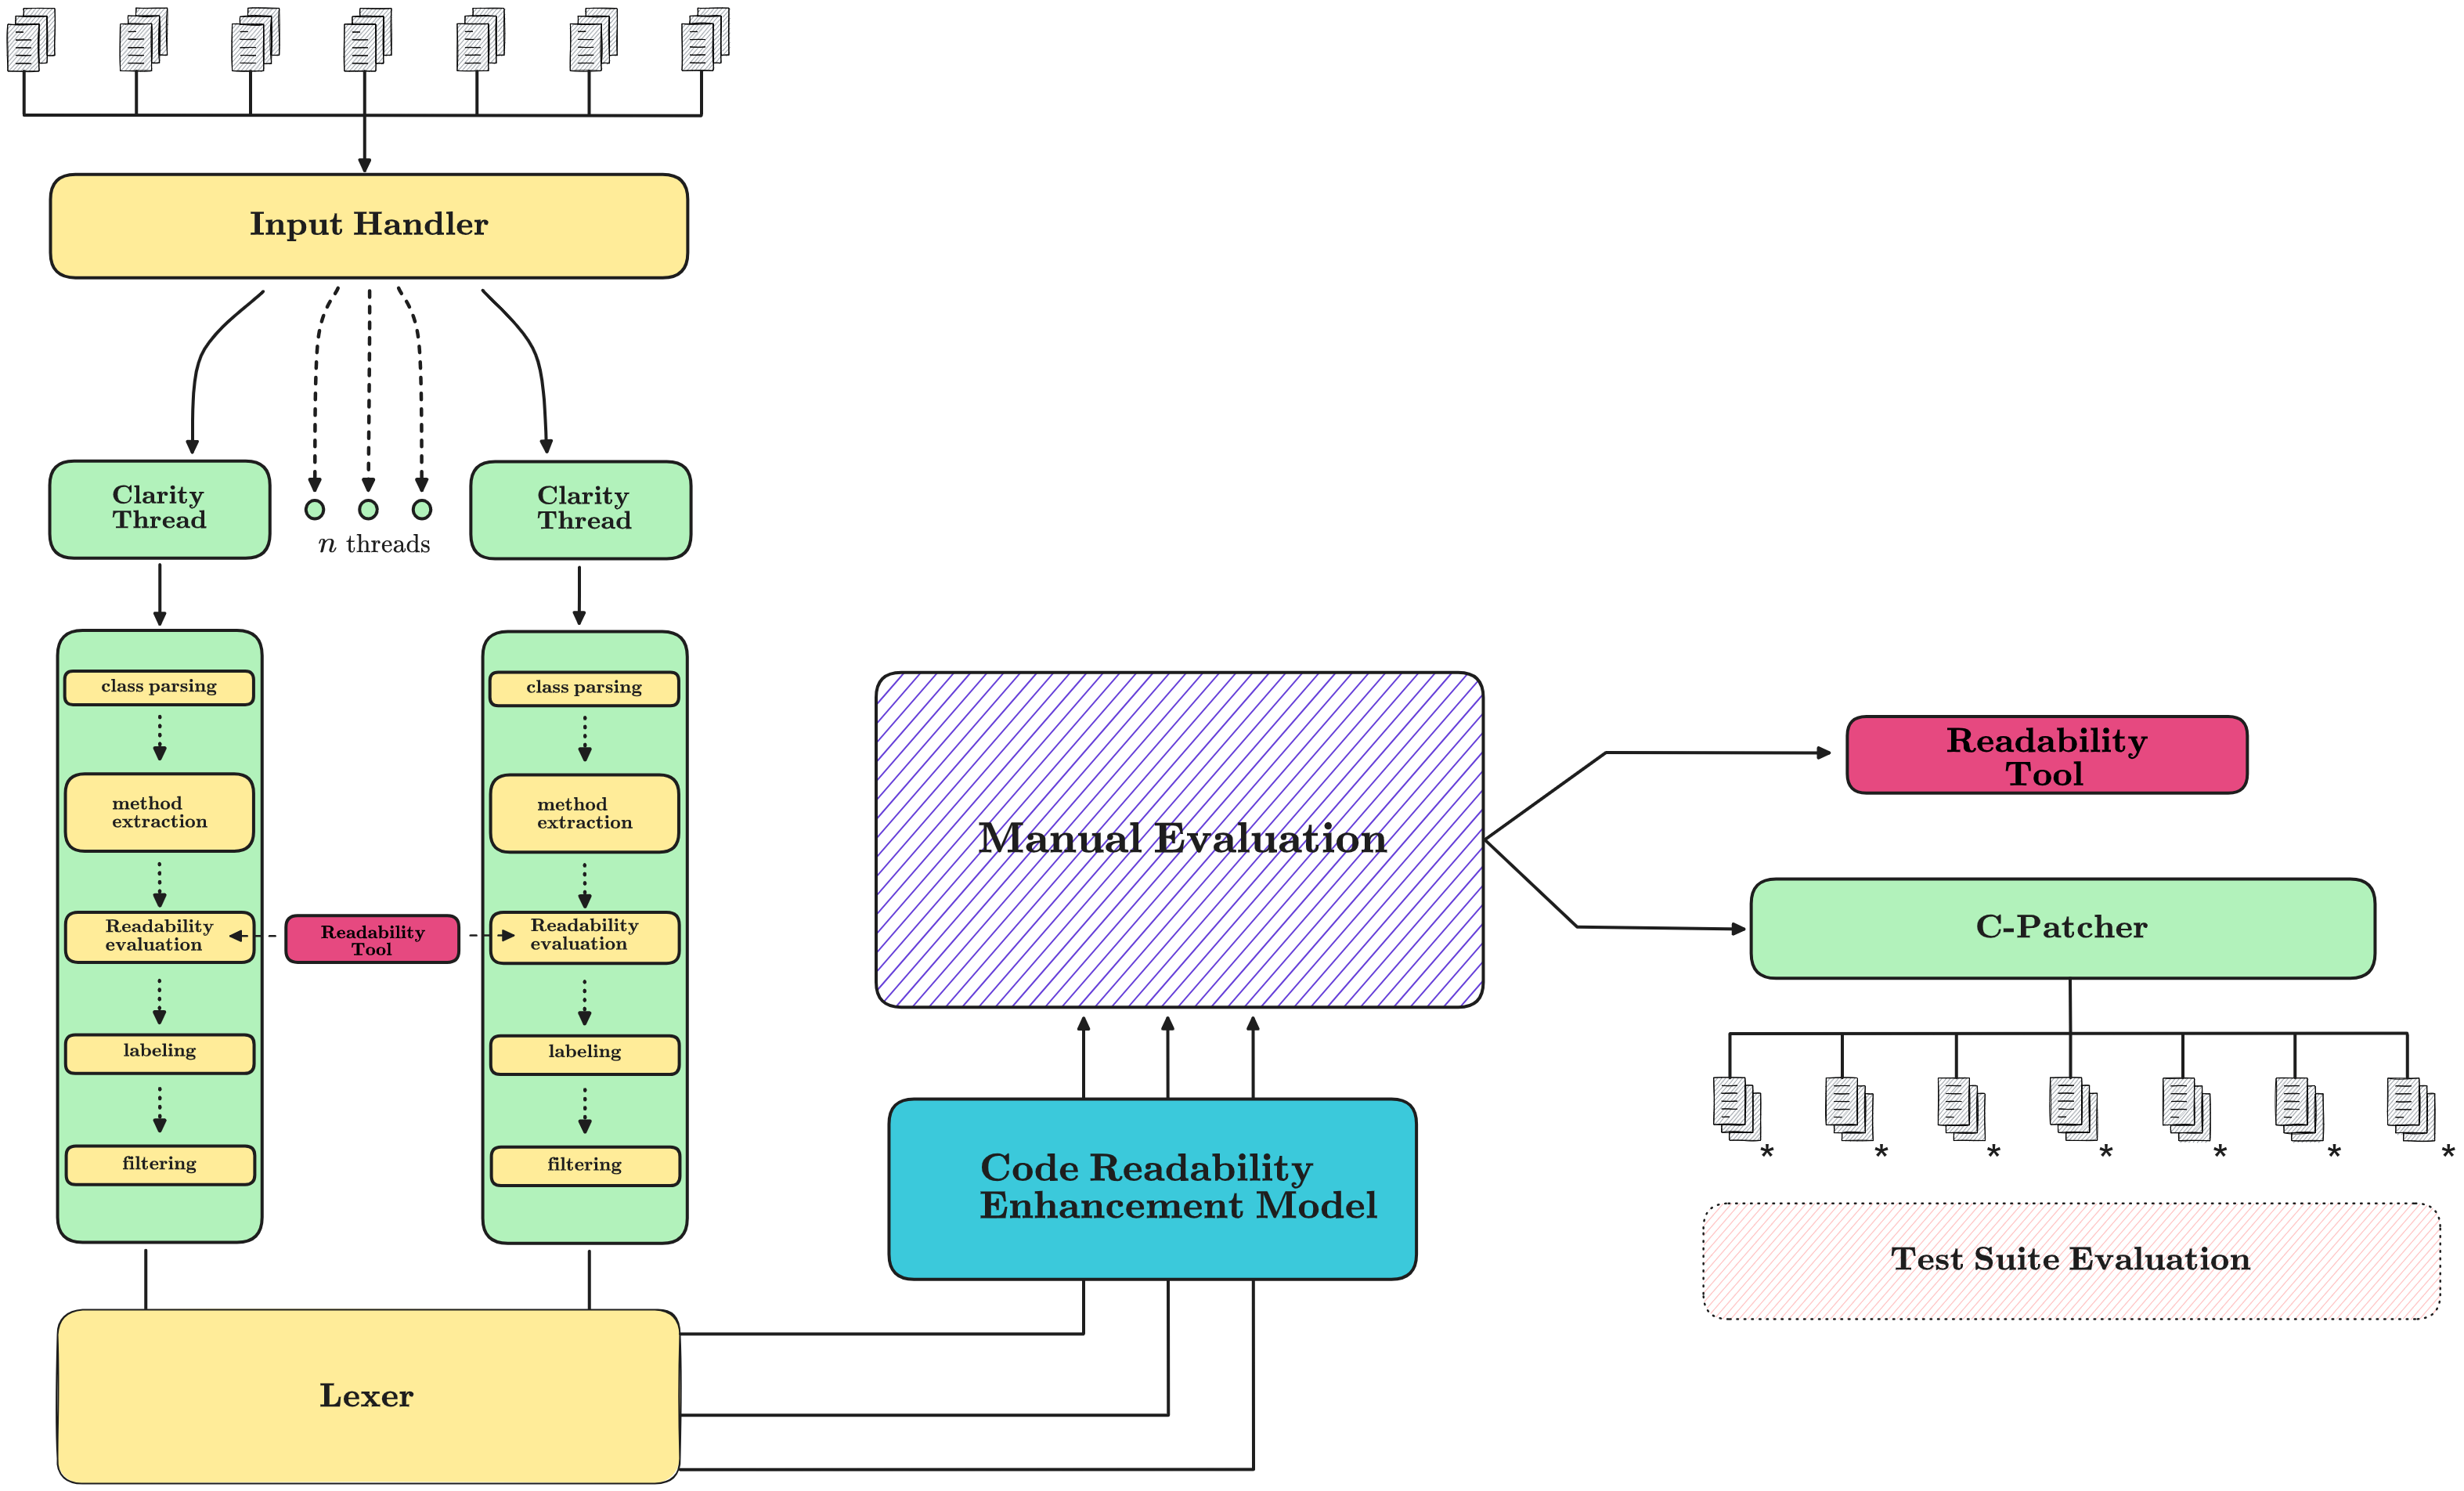
\includegraphics[width=1\textwidth,height=1\textheight,keepaspectratio]{figs/pipeline.png}
	\caption{}\label{fig:pipeline}
\end{figure}


\subsection{Data Collection}
In this phase, we utilized software repository mining techniques to extract the data essential for our research. We carefully selected three sizable Java projects, each actively maintained and equipped with a comprehensive test case suite. The chosen projects are:

\begin{itemize}
	\item \textbf{Guava}: an open source library from Google that provides a set of libraries useful for programming in Java;
	\item \textbf{Javaparser}: an open source library that allows you to analyze and manipulate Java source code;
	\item \textbf{Jenkins}: An open source automation system that provides support for building, testing, and deploying software.
\end{itemize}

\subsection{Data Preprocessing and Dataset Creation}
In this phase, our focus was on extracting methods from the selected projects. This approach was necessary because the insights gleaned from the Vitale et al. \cite{Vitale2023} study pertained specifically to Java code snippets, rendering reasoning at the class level impractical. To address this, we developed the "Clarity" tools, designed to extract methods from one or more Java projects, categorize them based on readability, and maintain a subset according to user-defined parameters. This tool comprises multiple components. Firstly, the Input Handler facilitates the analysis of multiple projects concurrently using multithreading techniques, primarily for optimization purposes. The Handler creates a set of threads corresponding to the number of input projects, with the user-defined numerical limit (defaulting to 4 threads) to prevent potential application crashes. Each thread executes a series of operations:

\begin{itemize}
	\item 1. \textit{Extract methods from java classes}
	\item 2. \textit{Evaluate methods readability }
	\item 3. \textit{Remove irrelevant results}
	\item 4. \textit{Labeling}
\end{itemize}
Which we will describe in detail in the next paragraphs.


\subsubsection{Methods Extraction} % (fold)
In this phase, we utilized the open-source tool \textit{Javaparser} to parse the Java classes, extracting the Abstract Syntax Tree (AST) a hierarchical representation of the structure of code that abstracts away details like spacing and formatting, which facilitated the identification of methods. From the extracted methods, we preserved crucial components including the declaration, body, annotations, and comments. Subsequently, as shown in Figure~\ref{code:dummy_class} this data was encapsulated within a dummy class and saved to file for further analysis.\newpage
\begin{lstlisting}[caption={Dummy Class}, label={code:dummy_class}, language = Java , frame = trBL , firstnumber = last , escapeinside={(*@}{@*)}]
public class DummyClass {
    //comments
    @Notation
    public void method() {
    }
}
\end{lstlisting}
To circumvent the extraction of "superfluous" methods, we implemented certain exclusions during this phase. Specifically, we chose to disregard getters and setters, as well as constructors. For the former two, we employed a heuristic based on the observation that getters and setters typically consist of no more than three lines. As for constructors, we leveraged the Javaparser API to identify and exclude them from the extraction process.
Although it is true that this heuristic may remove methods that are neither getters nor setters, we have still decided to use it. This decision is motivated by the fact that the likelihood of such methods containing readability errors is rather low, given the limited amount of code. Therefore, this explanation confirms the validity of the choice to exclude these methods.


\subsubsection{Readability Evaluation} % (fold)
\label{sub:Calculate readability}
To evaluate the readability of the Java methods, we utilized an API from a readability analysis tool developed as a result of the study conducted by Scalabrino et al. \cite{Scalabrino2018}. This tool offers an interface for analyzing the dummy classes generated during the extraction process. Through the analysis phase, by analyzing the code and taking into account different metrics such as line length, number of blank lines, periods etc. this tool produces a readability score \( s \) such that \( s \in [0,1] \), where:
\[
	\begin{aligned}
		0 & \implies \text{unreadable} \\
		1 & \implies \text{readable}
	\end{aligned}
\]
\newline
Once we obtained the score, we proceeded to save the necessary information for the tokenization and processing phase by the model. This data was saved in JSON format, retaining additional information required for later stages. Figure~\ref{code:method_info}is an example of the JSON structure:
\begin{lstlisting}[caption={Method's Information}, label={code:method_info}, language = json, frame = trBL , firstnumber = last , escapeinside={(*@}{@*)}]
{
  "name": "orNull",
  "method": "\t\t@Override\n\t\t@CheckForNull\n\t\tpublic T orNull(){\n\t\t    return null;\n\t\t}",
  "startLine": 64,
  "endLine": 68,
  "classPath": "guava/android/guava/src/com/google/common/base/Absent.java",
  "readabilityScore": 0.8923128247261047,
  "label": "NONE"
}
\end{lstlisting}
% subsection Calcolare la leggibilità (end)

\subsubsection{Data Filtering and Labeling} % (fold)
\label{sub:Labeling}
In the final phase of data extraction, considering the potentially vast number of methods generated by a large project, we opted to retain only a subset. Specifically, we selected the 20\% of the least readable methods, the 20\% of the average readable methods, and the 20\% of the most readable ones. To achieve this, we devised an algorithm that sorts the results based on the readability score and then filters out only the files meeting these percentage criteria. An example of the algorithm can be seen in Figure \ref{fig:filter_algorithm}.
As depicted, our decision was to retain not only the worst data, i.e., the least readable methods, but also the most readable and the averagely readable ones. This approach allows us to observe the model's performance across these three distinct scenarios.
\vspace{0.5cm}
\begin{figure}[H]
	\begin{center}
		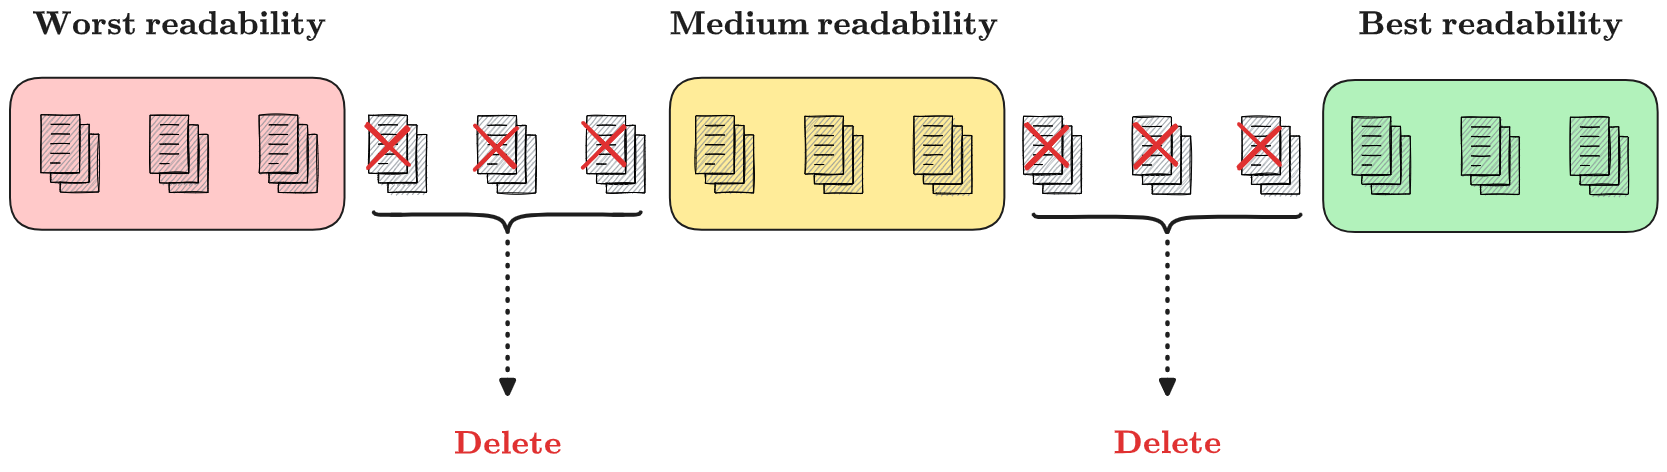
\includegraphics[width=0.95\textwidth]{figs/filter_algorithm.png}
	\end{center}
	\caption{}\label{fig:filter_algorithm}
\end{figure}


% subsection Labeling (end)
\subsubsection{Tokenization} % (fold)
\label{sub:Tokenization}
As mentioned, the model will take a series of methods as input and return an enhanced, more readable version. However, before proceeding with this, we need to pass our results through a lexer (lexical analyzer), which will enable us to divide the input text into meaningful sections known as tokens, representing the atomic units of the programming language. \newline
An example of tokenization is illustrated in the Table shown below:
\begin{table}[h!]
	\centering
	\begin{tabular}{|p{7cm}|p{7cm}|}
		\hline
		\textbf{Original Method}                      & \textbf{Tokenized Method}                                                                                                                                                                                                                                                                                                                                          \\
		\hline
		\begin{lstlisting}[language=Java, frame=none]
public void generate() {
    final int size = 0;
    final String alphabet = "";
    final String digits = "";
}
        \end{lstlisting} &
		\begin{lstlisting}[ frame=none]
public $whitespace$ void $whitespace$ generate ( ) $whitespace$ { $newline$ $indentation$ final $whitespace$ int $whitespace$ size $whitespace$ = $whitespace$ $number$ ; $newline$ $indentation$ final $whitespace$ string $whitespace$ alphabet $whitespace$ = $whitespace$ $string$ ; $newline$ $indentation$ final $whitespace$ string $whitespace$ digits $whitespace$ = $whitespace$ $string$ ; $whitespace$ 
        \end{lstlisting} \\
		\hline
	\end{tabular}
	\label{tab:tokenization}
	\caption{Comparison between the original method and the tokenized method.}
\end{table}
\newline
As evident, we eliminated extraneous characters such as spaces, newlines, and tabs, which convey text positioning but hold no significance for the language. Instead, we replaced them with specific tokens representing their behavior. Subsequently, we apply the theory described above to the set of JSON files obtained from the preceding steps to generate the input file for the model. The Ruby program responsible for the tokenization phase will generate, at the end, the Dataset in the form of a \textbf{\textit{TSV}} file.

\subsection{Model Application} % (fold)
In this phase, we processed the data obtained in previous phases using the deep learning model provided by Vitale et al. \cite{Vitale2023}. The model was accessible via a collaborative environment called \textit{Colab}, enabling the execution of Python instructions to configure the model and extract relevant data from the \textit{.tsv} file. Specifically, we focused on the \textit{tokenized\_method} field, containing the tokenized method, which served as input for the model. The model processed this data and returned a new tokenized method with readability changes, which we subsequently inserted back into the \textit{.tsv} file under a field named \textit{model\_prediction}\newline

\subsection{Data analysis} % (fold)
\label{sec:Data analysis}

From this point onward, we were almost equipped to address research questions \textit{RQ1} and \textit{RQ2}. We initiated an analysis of the data obtained to address these questions, starting with a manual evaluation of the model's responses to validate the results and ascertain if the model had indeed altered the instances. During this manual review phase, for the methods modified by the model, we manually replaced tokens that couldn't be automatically replaced, such as \textbf{\$string\$} and \textbf{\$number\$}. This manual replacement was necessary as the output of the model is not deterministic, thus making it impossible to automatically predict which string or number corresponds to which token. Additionally, during this manual phase, we also adjusted strings that were previously in uppercase, as the model, as currently defined, only provides predictions in lowercase.\newline
During this manual analysis, certain observations were made, and consequently, noticing a similar pattern in each modification, we decided to preserve a relatively small subset of the analyzed methods. Indeed, the total number (again 20\% of the total methods) amounted to approximately 5,000 methods per project. This number would have resulted in the need to manually analyze over 15,000 methods. To make the task more manageable, we decided to retain a sample of 100 methods per project. Additionally, to facilitate the modification of these methods, we decided to create a series of methodologies.
\begin{itemize}
	\item In series model result detokenization.
	\item Automatic camelCase conversion.
\end{itemize}
To address \RQ{1}, we needed to analyze the code provided by the model using Scalabrino \etal \cite{Scalabrino2018} tool. To accomplish this, we applied the detokenization phase, which was divided into two parts. The first part, automatic, dealt with replacing all tokens that could be replaced without manual intervention, such as \textbf{\$newline\$} or \textbf{\$indentation\$}. The second part was manual because we had to remove all tokens that could not be removed automatically. To facilitate this procedure, we introduced the first methodology which helped automate a component of this manual phase, namely the dataset manipulation. The second methodology was employed to expedite the process and reduce the manual effort required. By implementing this procedure, we decreased the potential for manual error introduction. This methodology, shown in Figure~\ref{fig:To camelCase algorithm}, involved converting the methods into CamelCase format. We developed a parser that generated a binary tree from the method under analysis. The algorithm precisely divides the input string into a list of strings using space as a delimiter and performs the following operations for each string:
\begin{itemize}
	\item 1. Set the string as the root of the tree.
	\item 2. Iterate through the string character by character, from left to right.
	\item 3. If we encounter a punctuation mark, set that mark as the root of the tree and the string preceding the mark as the left leaf. Then set the right node with the remaining unanalyzed string and recursively call the procedure on that node.
\end{itemize}
As we can observe, this algorithm defines an invariant that we can exploit to isolate words devoid of punctuation marks. Indeed, it will always be true that words lacking such marks will be found, for each subtree, either in a left leaf or at the root position. With this established, it was straightforward to reconstruct the original string by isolating the words that needed to be converted into CamelCase. For the conversion, we used a Python library called \textit{ninjaword}, which, employing a \textbf{N}atural \textbf{L}anguage \textbf{P}rocessing approach, successfully converted the strings into CamelCase with a reasonable success rate. It is worth noting that this library still has limitations. For example, the word "lightinglobe" can be correctly decomposed into multiple words, all equally valid: ["lighting", "globe"] or ["light", "in", "lobe"]. This highlights that, although this approach was simplifying in some respects, it certainly did not eliminate the need for manual analysis. Additionally, it's worth noting that this approach did not handle a certain type of keywords such as non-primitive data types since those types in Java start with an uppercase letter.
\begin{figure}[H]
	\begin{center}
		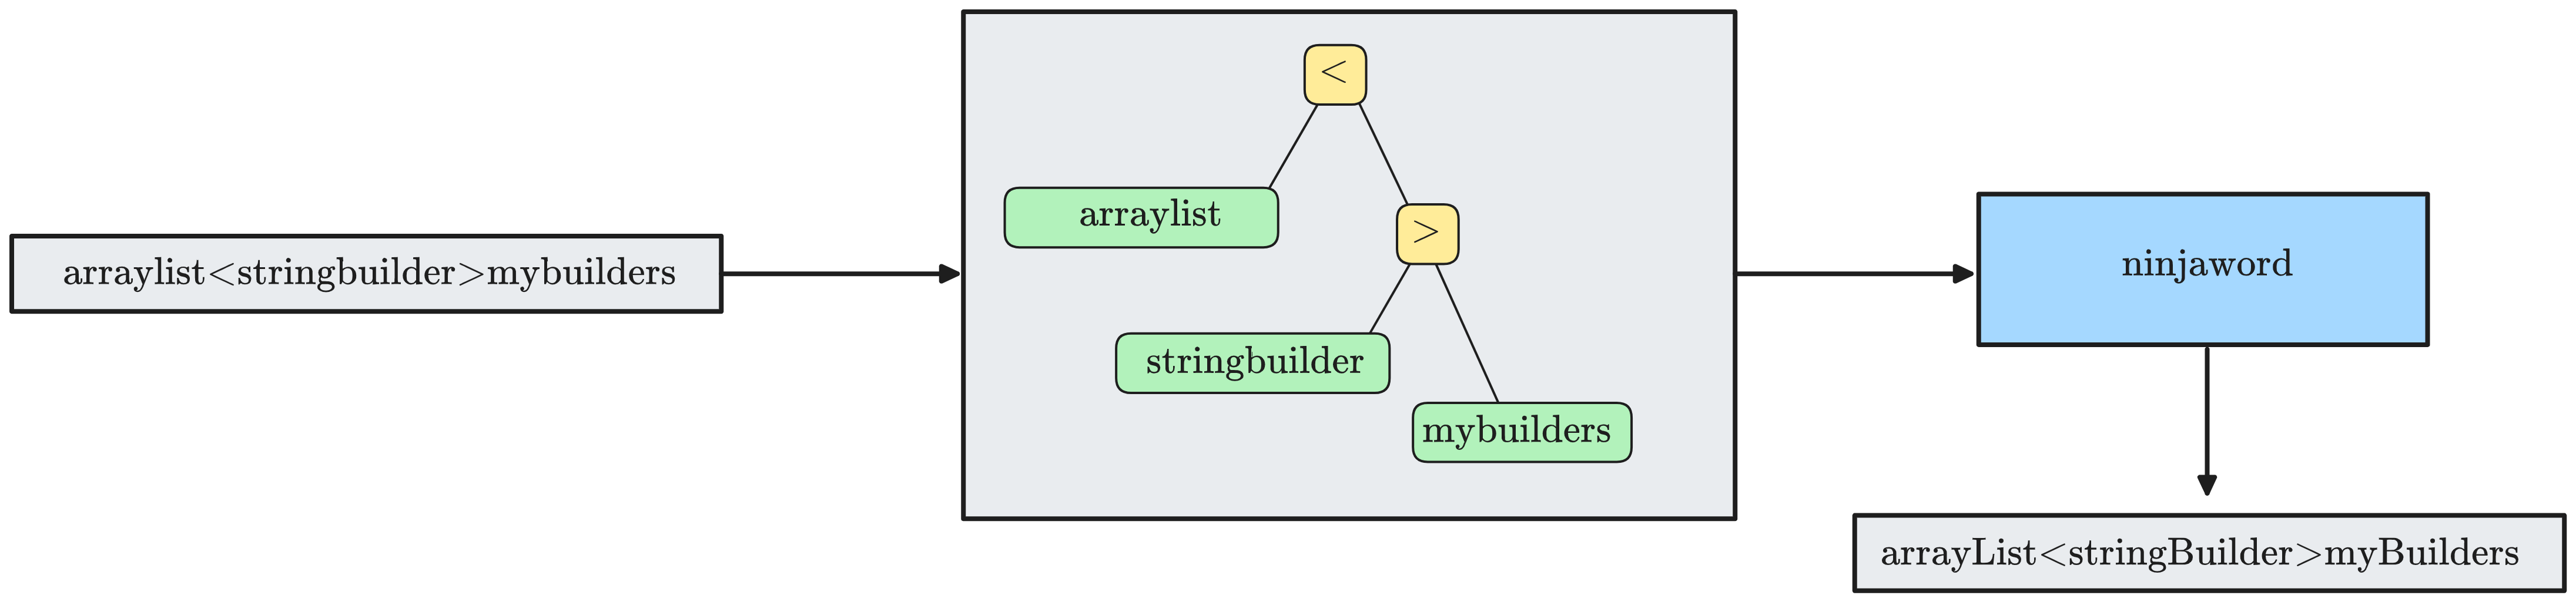
\includegraphics[width=0.95\textwidth]{figs/clay.png}
	\end{center}
	\caption{}\label{fig:To camelCase algorithm}
\end{figure}
The manual analysis removed a significant portion of the methods.
\begin{itemize}
	\item \textbf{Guava}: 67/100 methods were considered faulty
	\item \textbf{Jenkins}: 58/100 methods were considered faulty
	\item \textbf{Javaparser}: 58/100 methods were considered faulty
\end{itemize}
During this manual analysis, we corrected the syntax of certain methods by replacing tokens and rewriting procedures using the camelCase convention. Throughout this phase, we disregarded methods that were not modified by the model and discarded those deemed faulty. With "faulty," we mean that the method was not correctly modified by the model, thus resulting in syntax errors or even semantic errors, such as using an undeclared variable or omitting to return a value. \newline
During this analysis phase, we also manually indented the results. This was necessary because the model was trained in such a way that it could not distinguish 4-space indentations rather than 8-space indentations for the token \textbf{\$indentation\$}. However, this manual indentation did not significantly alter the model's output; rather, it ensured that each statement was properly aligned. This precaution was taken to prevent misinterpretations by the Scalabrino et al. tool \cite{Scalabrino2018}, and to ensure a more comfortable visualization.\\
We then executed Scalabrino \etal \cite{Scalabrino2018} tool to evaluate model prediction readability, and subsequently conduct a manual readability analysis, the objective was twofold: to identify minimal differences that the tool might have overlooked and to provide a secondary assessment of readability based on insights drawn from the work of Fakhoury et al. \cite{Fakhoury2019}. However, this secondary analysis does not rely on specific metrics but rather on perceived improvements as evaluated by the developer, namely myself. To address question \RQ{2}, we conducted a patching phase. Leveraging information about the class membership and the location of a given method within that class, obtained during the method extraction phase, it was straightforward to replace the original methods with the modified ones. Subsequently, we executed the test suite of the projects to understand if and how these changes impacted the functionality of the procedure. The execution of the test cases was atomic for each method, which means that, to prevent the modification of one method from impacting the results of another, we executed the test suite at every iteration of the patching procedure. This allowed us to determine whether the code behavior had been altered. The results of these analyses, along with other considerations, are reported in the next chapter.
% section Data analysis (end)


\chapter{Results}
\label{Chapter4}

In this section, the results obtained from the analysis conducted on the various systems, namely \textbf{\textit{Javaparser}}, \textbf{\textit{Jenkins}}, and \textbf{\textit{Guava}}, are presented. The results were obtained through the analysis of two main aspects: the readability of the code and the correctness of the test cases. Specifically, regarding the readability of the code, the average differences calculated by the Scalabrino et al. \cite{Scalabrino2018} tool before and after the application of the model were considered. Regarding the correctness of the test cases, the results obtained from the analysis conducted, individually for each method, on the respective systems' test suites injected with the methods modified by the model were considered.\newline \newline
Let's consider the results produced by the analysis on the systems, as shown in the Table \ref{tab:results}.
\begin{table}[h!]
	\centering
	\resizebox{\textwidth}{!}{%
		\begin{tabular}{@{}p{2cm}ccp{4cm}p{3cm}cc@{}}
			\toprule
			\textbf{System}             & \textbf{Label} & \textbf{N. of Methods} & \textbf{Avg. Readability Score Diff.}                     & \textbf{N. of Test Passed} & \textbf{Avg. Manual Readability Score}                    \\
			\midrule
			\multirow{3}{*}{Jenkins}    & LOW            & 14                     & -0.0049 \begingroup\color{red}\blacktriangledown\endgroup & \%21.42 (3/14)             & 0                                                         \\
			                            & MID            & 8                      & 0.0187  \begingroup\color{green}\blacktriangle\endgroup   & \%37.50 (3/8)              & -0.0375 \begingroup\color{red}\blacktriangledown\endgroup \\
			                            & HIGH           & 18                     & -0.0008 \begingroup\color{red}\blacktriangledown\endgroup & \%77.77 (14/18)            & 0                                                         \\
			\midrule
			\multirow{3}{*}{Javaparser} & LOW            & 26                     & 0.0308 \begingroup\color{green}\blacktriangle\endgroup    & \%3.84 (1/26)              & 0.0884 \begingroup\color{green}\blacktriangle\endgroup    \\
			                            & MID            & 13                     & -0.0096 \begingroup\color{red}\blacktriangledown\endgroup & \%38.46 (5/13)             & 0.0076 \begingroup\color{green}\blacktriangle\endgroup    \\
			                            & HIGH           & 3                      & -0.0132 \begingroup\color{red}\blacktriangledown\endgroup & \%0.0 (0/3)                & 0                                                         \\
			\midrule
			\multirow{3}{*}{Guava}      & LOW            & 18                     & 0.0173 \begingroup\color{green}\blacktriangle\endgroup    & \%100.0 (18/18)            & 0.0111 \begingroup\color{green}\blacktriangle\endgroup    \\
			                            & MID            & 13                     & 0.0369 \begingroup\color{green}\blacktriangle\endgroup    & \%100.0 (13/13)            & 0.0923  \begingroup\color{green}\blacktriangle\endgroup   \\
			                            & HIGH           & 2                      & -0.0625 \begingroup\color{red}\blacktriangledown\endgroup & \%100.0 (2/2)              & -0.1   \begingroup\color{red}\blacktriangledown\endgroup  \\
			\bottomrule
		\end{tabular}%
	}
	\caption{Analysis results}
	\label{tab:results}
\end{table} \newpage
\section{RQ1: Code Readability Improvement}
The readability results indicate that the model by Vitale et al. \cite{Vitale2023} performs well with poorly and moderately readable methods, offering a slight improvement in readability. It's important to note that the model was trained on diff lines rather than at the method level. Therefore, when conducting this type of analysis, results may deviate from the training set, leading to outcomes like these. The results presented in Table \ref{tab:results} are particularly interesting as they demonstrate the best outcomes regarding moderately readable methods. For poorly readable methods, we can observe that the average readability improvement is higher for the Javaparser system (see Table \ref{tab:results}). The only tangible negative results (an average decrease in readability) are observed for methods classified as highly readable.\\
An example of this could be as follows:
\begin{lstlisting}[language = Java ,caption={Original Method}, frame = trBL , firstnumber = last , escapeinside={(*@}{@*)}]
@Override
public int hashCode(){
    int result = kind;
    result = 31 * result + text.hashCode();
    return result;
}
\end{lstlisting}
\begin{lstlisting}[language = Java , caption={Modified Method},frame = trBL , firstnumber = last , escapeinside={(*@}{@*)}]
@Override 
public int hashCode(){ 
   int result = kind.toString(); 
   result = 31 * result + text.hashCode(); 
   return result; 
}
\end{lstlisting}
As observed, the decrease in readability (-0.06) can be attributed to the addition of the \texttt{toString()} method to the variable \texttt{kind}. Regarding readability, we conducted further manual analysis on instances, assessing the improvement or deterioration in readability of the changes made by the model using a score ranging from -1 to 1. We then reported the median score in Table \ref{tab:results}. The average of the manual scores and the average difference in readability are two indicators that can indeed be compared, as they were calculated using the same scale. However, they should be interpreted with caution as the manual evaluation was not conducted following specific metrics but rather based on personal assessment. That being said, we can observe that this average aligns with the average difference in readability suggested by the tool developed Scalabrino \etal \cite{Scalabrino2018} deviating only slightly for one of the cases. Although not apparent from the average, there are instances where the model significantly improved the readability of the methods, and such improvement is also reflected in the manual assessment. Take the following example:
\begin{lstlisting}[language = Java ,caption={Original Method}, frame = trBL , firstnumber = last ,label={code:original_method}, escapeinside={(*@}{@*)}]
private void generateVisitMethodForNode(BaseNodeMetaModel node, ClassOrInterfaceDeclaration visitorClass, CompilationUnit compilationUnit){
    final Optional<MethodDeclaration> existingVisitMethod = visitorClass.getMethods().stream().filter(m -> "visit".equals(m.getNameAsString())).filter(m -> m.getParameter(0).getType().toString().equals(node.getTypeName())).findFirst();
    if (existingVisitMethod.isPresent()) {
        generateVisitMethodBody(node, existingVisitMethod.get(), compilationUnit);
    } else if (createMissingVisitMethods) {
        MethodDeclaration newVisitMethod = visitorClass.addMethod("visit").addParameter(node.getTypeNameGenerified(), "n").addParameter(argumentType, "arg").setType(returnType);
        if (!visitorClass.isInterface()) {
            newVisitMethod.addAnnotation(new MarkerAnnotationExpr(new Name("Override"))).addModifier(PUBLIC);
        }
        generateVisitMethodBody(node, newVisitMethod, compilationUnit);
    }
}
\end{lstlisting}
\begin{lstlisting}[language = Java ,caption={Modified Method}, frame = trBL , firstnumber = last ,label={code:Prediction Method}, escapeinside={(*@}{@*)}]
private void generateVisitMethodForNode(BaseNodeMetaModel node, ClassOrInterfaceDeclaration visitorClass CompilationUnit compilationUnit) { 
   final Optional<MethodDeclaration>existingVisitMethod = visitorClass getMethods().stream() 
       .filter(m-> "visit" equals(m.getNameAsString())) 
       .filter(m-> m.getParameter(0).getType().toString().equals(node.getTypename())) 
       .findFirst(); 
   if (existingVisitMethod isPresent()) { 
       onVisitMethodBody(node, existingVisitMethod get(), compilationUnit); 
   } else if (createMissingVisitMethods) { 
       onVisitMethodBody(node, newVisitMethod compilationUnit); 
   } 
} 
\end{lstlisting}
Although the model removed the nested \texttt{if(...)} statement within the \texttt{else if ()\{...\}} construct, it intriguingly split the various \texttt{.filter()} and \texttt{.findFirst()} statements across multiple lines, significantly enhancing readability. In fact, in this instance, the readability improvement amounts to 0.5 compared to the original code, a result that mirrors the increase of 1 assigned in my manual assessment. Furthermore, this enhancement was observed for an instance initially considered to have low readability. Another noteworthy improvement, albeit minor, is evident in the \texttt{castValue} method of \textbf{\textit{Javaparser}}:
\begin{lstlisting}[language = Java , caption={Original Method}, frame = trBL , firstnumber = last , escapeinside={(*@}{@*)}]
public static String castValue(String value, Type requiredType, String valueType){
    String requiredTypeName = requiredType.asString();
    if (requiredTypeName.equals(valueType))
        return value;
    return String.format("(%s) %s", requiredTypeName, value);
}
\end{lstlisting}
\begin{lstlisting}[language = Java , caption={Modified Method},frame = trBL , firstnumber = last , escapeinside={(*@}{@*)}]
public static String castValue(String value, Type requiredType, String valueType) { 
   String requiredTypeName = requiredType.asString(); 
   if (requiredTypeName.equals(valueType)) { 
       return value; 
   } 
   return string.format("(%s) %s", requiredTypeName, value); 
}
\end{lstlisting}
As we can observe, the only modification made was the addition of curly braces within the \texttt{if()} statement, effectively enhancing the clarity of the statement's block separation. An example of a decrease in readability is evident in  this \textbf{\textit{Guava}} method, named \texttt{tryDrainReferenceQueues()}
\begin{lstlisting}[language = Java ,caption={Original Method}, frame = trBL , firstnumber = last , escapeinside={(*@}{@*)}]
void tryDrainReferenceQueues(){
  if (tryLock()) {
      try {
          drainReferenceQueues();
      } finally {
          unlock();
      }
  }
}
\end{lstlisting}
\begin{lstlisting}[language = Java , caption={Modified Method},frame = trBL , firstnumber = last , escapeinside={(*@}{@*)}]
void tryDrainReferenceQueues() { 
   drainReferenceQueues(); 
   if (tryLock()) { 
       drainReferenceQueues(); 
   } 
}
\end{lstlisting}
In this example, we notice a reduction in the number of lines of code, at the expense of procedural clarity, thus making the operation \texttt{drainReferenceQueues()} more ambiguous. As we see, the modifications to readability have been made in a subtle manner, and in some cases, they have not been made at all. However, the model has demonstrated the ability to enhance readability and, in some instances, provide a noticeable improvement. Nevertheless, such enhancements are, all in all, occasional, and on average, the fluctuations in improvement are relatively limited.



\section{RQ2: Behavior Changes} % ()
The results demonstrate how the model tends to negatively alter the behavior of poorly readable methods. For moderately readable methods, it is observed that in 62\% of cases, correctness is compromised. Regarding highly readable methods, the model, on average, does not compromise their functionality. In a specific case, namely the \textbf{\textit{Guava}} system (see Table \ref{tab:results}), it is observed that the model did not compromise the correctness of the methods, however, this result contradicts some instances observed for this system, casting doubt on the patching operation and the execution of the respective test cases for this particular instance. Another particularly important aspect to consider is the presence of a relatively low subset of methods compared to the originally considered 300. In fact, more than half of these (193/300) were deemed faulty during the manual analysis due to obvious syntactic and/or semantic errors. These values suggest that this model tends to compromise the majority of the analyzed methods.
The reasons for such compromise are of various natures. For example, incorrect repositioning of parentheses clearly creates a syntactic error that prevents the method from being executed. Other times, however, the model exhibits anomalous behaviors in modification, completely altering the structure of the original method:
\begin{lstlisting}[language = Java , caption={Original Method},frame = trBL , firstnumber = last , escapeinside={(*@}{@*)}]
		private static void explode(File archive, File destDir) throws IOException{
		    Util.createDirectories(Util.fileToPath(destDir));
		    // timestamp check
		    File explodeTime = new File(destDir, ".timestamp2");
		    if (explodeTime.exists() && explodeTime.lastModified() == archive.lastModified())
		        // no need to expand
		        return;
		    // delete the contents so that old files won't interfere with new files
		    Util.deleteRecursive(destDir);
		    try {
		        Project prj = new Project();
		        unzipExceptClasses(archive, destDir, prj);
		        createClassJarFromWebInfClasses(archive, destDir, prj);
		    } catch (BuildException x) {
		        throw new IOException("Failed to expand " + archive, x);
		    }
		    try {
		        new FilePath(explodeTime).touch(archive.lastModified());
		    } catch (InterruptedException e) {
		        // impossible
		        throw new AssertionError(e);
		    }
		}
\end{lstlisting}
\newpage
\begin{lstlisting}[language = Java , caption={Modified Method},frame = trBL , firstnumber = last , escapeinside={(*@}{@*)}]
	 private static void explode(file archive, file destdir) throws ioexception { 
       util.createdirectories (util.filetopath (destdir)); 
       midnight = new file (destdir, $string$); 
       if (reportedtime.exists () && explodetime.lastmodified () == archive.lastmodified ()) 
           //////.get-------------------------------------------------------------------------------------------------------------------------------------------------------------------------------------------------------------------------------------------------------------------------------------------------------------------------------------
\end{lstlisting}
We can observe another example of this behavior even in this instance:
\begin{lstlisting}[language = Java , caption={Original Method},frame = trBL , firstnumber = last , escapeinside={(*@}{@*)}]

private int nextOutputChar() throws IOException{
    int next = nextInputChar();
    switch(next) {
        case EOF:
            return EOF;
        case BACKSLASH:
            {
                if (_backslashSeen) {
                    return clearBackSlashSeen(next);
                }
                return backSlashSeen();
            }
        default:
            {
                // An arbitrary character.
                return clearBackSlashSeen(next);
            }
    }
}
\end{lstlisting}
\begin{lstlisting}[language = Java , caption ={Modified Method}, frame = trBL , firstnumber = last , escapeinside={(*@}{@*)}]
private int nextoutputchar () throws ioexception { 
     int next = nextinputchar () ; 
     switch (next) { 
         case eof : 
         return eof ; 
         case backslash : 
     { 
     if (_backslashseen) { 
         return clearbackslashseen (next) ; 
     } 
     return backslashseen () ; 
     } 
     default : 
     { 
     $//g$an143示示 
     return clearbackslashseen (next) ; 
     } 
}
\end{lstlisting}
And in some cases, it has removed instructions necessary for the functioning of the method, as in this example where the \textit{return} statement is removed:
\begin{lstlisting}[language = Java , caption={Original Method}, frame = trBL , firstnumber = last , escapeinside={(*@}{@*)}]
@Deprecated
private static T handleResult(ParseResult<T> result){
    if (result.isSuccessful()) {
        return result.getResult().get();
    }
    throw new ParseProblemException(result.getProblems());
}
\end{lstlisting}
\newpage
\begin{lstlisting}[language = Java , caption={Modified Method}, frame = trBL , firstnumber = last , escapeinside={(*@}{@*)}]
@deprecated 
 private static t handleresult(parseresult <t> result) { 
     if (! result.issuccessful()) { 
         throw new parseproblemexception(result.getproblems()); 
     }
\end{lstlisting}
In these examples, we notice that the strings are not in CamelCase, and the tokens \textbf{\$string\$} and \textbf{\$number\$} have not been replaced. This is because this phase has never been applied given the presumably flawed nature of the model's modification. As we can see, some procedures have been invalidated by purely syntactic changes. However, there have also been logical changes that went unnoticed during the initial analysis but were later discovered during the examination of the modifications made by executing the test suite of the respective projects. We can observe this behavior, for example, in the method \texttt{lookupFirst()} of \textbf{\textit{Jenkins}}:
\begin{lstlisting}[language = Java , caption={Original Method},frame = trBL , firstnumber = last , escapeinside={(*@}{@*)}]
@NonNull
public static U lookupFirst(Class<U> type){
  var all = lookup(type);
  if (!all.isEmpty()) {
      return all.get(0);
  } else {
      if (Main.isUnitTest) {
          throw new IllegalStateException("Found no instances of " + type.getName() + " registered (possible annotation processor issue); try using `mvn clean test -Dtest=…` rather than an IDE test runner");
      } else {
          throw new IllegalStateException("Found no instances of " + type.getName() + " registered");
      }
  }
}
\end{lstlisting}
\begin{lstlisting}[language = Java , caption={Modified Method},frame = trBL , firstnumber = last , escapeinside={(*@}{@*)}]
 @NonNull 
 public static U lookupFirst(Class<U> type) { 
     if (!all.isEmpty()) { 
         throw new IllegalStateException("Found no instances of " +type.getName()+ " registered(possible annotation processor issue); try using `mvn clean test -Dtest=…` rather than an IDE test runner"); 
     } 
     if (Main.isUnitTest) { 
         throw new illegalStateException("Found no instances of " +type.getName()+ " registered"); 
     } 
 }
\end{lstlisting}
Moreover, we also observe an increase in readability of 0.4 compared to the original method. We can see that the method has been streamlined by the improvement operation (which explains the increase in readability performed by the model); however, this has compromised correctness, thus undermining the refactoring operation. \\ In general, the majority of instances are represented by results of this kind, although in some cases, this does not occur. It is clear that although enticing, the model is not yet able to offer an acceptable accuracy to be considered a valid approach to automated refactoring. Nevertheless, it remains extremely promising.










% section Risultati sui casi di testj (end)


\chapter{Threats to Validity}
\label{Chapter5}

It is crucial to acknowledge potential threats to the validity of an experiment. Firstly, it's important to clarify that the evaluation of readability results, both before and after modification, relies on a heuristic-based tool. While this evaluation may not be mathematically precise, it holds significant statistical value. This aspect is pivotal as much of the experiment hinges on these heuristics; hence, any inaccuracies in them could significantly impact the results. Another potential threat to validity arises from the experiment's reliance on a relatively small sample of projects. Consequently, we lack sufficient data to deem the results statistically representative. However, this serves as a solid starting point, as it underscores the genuine potential of such models, albeit in a limited capacity. \newline \newline A potential threat to the validity of the study lies in the fact that a significant portion of the entire analysis relies on manual validation. This manual evaluation played a crucial and substantive role, given that the model, at the time of publication, only has the capability of outputting in lowercase. Therefore, this phase has played an important part in the study, and it is possible that this validation may have introduced errors that could have influenced the results. \newline Another threat to the validity of the study arises from the fact that the results regarding the correctness of the methods were obtained through the analysis of the test suite. This may not be sufficient to guarantee the correctness of the code, as such a test suite may not cover all possible scenarios in which a bug can be introduced.

\chapter{Conclusion and Future Work}
\label{Chapter6}
As observed during this experimental study, the potential for applying machine learning techniques is undoubtedly high, but the results are still nascent. Indeed, although these techniques could significantly impact the software development industry, it is clear that such an impact may require time to mature. Nevertheless, this experimental thesis has provided a pipeline of operations and a dataset that could be valuable for future studies. Future work will focus on applying the pipeline defined in this study on the next iterations of the model, which will not have the same limitations as the current model. In addition, future work could focus on various aspects, such as applying these techniques to other programming languages and analyzing the behavior of future versions of the model considered in the study. In addition to this, future work could extend this research by using a larger amount of data compared to what we utilized in the analysis phases.




%---------------------------------------------------------------------------------
%	BIBLIOGRAPHY
%---------------------------------------------------------------------------------
\newpage
\printbibliography[heading=bibintoc]


%---------------------------------------------------------------------------------
% Thanksgivings
%---------------------------------------------------------------------------------
\newpage
\thispagestyle{plain}
\noindent {\LARGE \textbf{Ringraziamenti}}
\vspace{.05\textheight}

\noindent Vorrei dedicare le prossime righe a tutte le persone che mi hanno sostenuto, direttamente o indirettamente, durante il mio percorso di vita.
\newline\newline
Voglio ringraziare la mia famiglia, con tutto il cuore. Quando decisi di intraprendere questo percorso, di virare dalla rotta da me precedentemente considerata, voi ci siete stati e mi avete sostenuto, in tutti i sensi. Non potete sentire ciò che sento perché l'empatia è l'illusione di provare ciò che un'altra persona prova, ma sappiate che, nel momento in cui sto scrivendo questa dedica, e in tantissimi dei momenti che hanno caratterizzato questo viaggio, ho e ho avuto il cuore ricolmo di gratitudine. Grazie.
\newline\newline
Ti ringrazio Cox per avermi spalleggiato in questo lungo context switch e per avermi spronato, in via indiretta, a dare il meglio di me. Ti ringrazio per avermi offerto un infanzia degna di essere vissuta e soprattutto, di esserti preso la parte più noiosa dello sviluppo software! <Kiss><Kiss> Ringo
\newline\newline
(M)artina, che dire, ti dico grazie perché mi sei sempre stata accanto, con il tuo fare giocoso hai ispirato il meglio in me. Ora sono come una primogem che cade dal cielo... con che colore mi vedi? Nah, non importa, sappi che quello che penso di te è e sarà sempre questo: Sei una persona speciale e ti voglio e vorrò sempre bene, qualunque cosa tu faccio, dovunque tu sia.
\newline\newline
Mamma, voglio ringraziarti per quello che hai fatto e per quello che fai tutti i giorni per me. La vita ci ha offerto alti e bassi, e nonostante tutto tu sei stata in grado di risorgere da ogni caduta. Ti ammiro per la tua tenacia, perché non è una qualità da poco. Da te ho ricevuto tanto, l'affetto di una madre, la comprensione di una madre e l'insegnamento che tutto, in fin dei conti, può essere messo in dubbio!. Ti voglio un mondo di bene.
\newline\newline
Papà, voglio ringraziarti con tutto il cuore, non sono un grande scrittore, ma spero che le mie poche parole sgrammaticate possano farti capire quanto io sia fiero di te. Sei la persona che ha e continua ad ispirare la mia vita e penso che questo sia tutto ciò che un padre possa mai volere. Ti ringrazio per il tuo sostegno costante, per la tua capacità di capirmi e per la tua immancabile grinta che ha fatto di me ciò che sono ora. Ti voglio un mondo di bene.
\newline\newline
Voglio ringraziare tutti i miei zii, zie, cugini e cugini. Siete parte di ciò che ha contribuito a rendere me ciò che sono ora e grazie al vostro sostegno e affetto, ho vissuto grandi momenti. Siete una parte importante, una parte che associo sempre alla festa e ai momenti felici. Vi ringrazio per essere rimasti coesi gli uni con gli altri perché, grazie a voi, ho potuto apprezzare a pieno il concetto di famiglia.
\newline\newline
Voglio ringraziare anche te Sonia! Si si, ora ti faccio piangere un po'! Già fatto? È stato facile. Sul serio, magari pensi di non esserlo stato ma lascia che ti contraddica, sei stata davvero importante per me. Grazie per avermi offerto cosi tanto, senza che io potessi fare altrettanto per te. Sappi che mi ricordo di tutto il bene che ricevo. Sei una persona vera, una Donna vera (altro che rose villein!) e sono contento di poter apprezzare la tua grazia e fermezza da cosi vicino. Ti voglio tanto bene.
\newline\newline
Ai miei nonni, vi voglio bene e vi ringrazi per aver creduto in me. La distanza non vi ha impedito di dimostrarmi il vostro affetto e appoggio. Nonna ti ringrazio per tutto quello che mi hai dato: un letto dove dormire, tanto amore e pranzi e cene buonissime. Sei un'artista in quello che fai, oltre che una nonna esemplare, e sappi che io ti voglio e vorrò sempre un mondo di bene. Nonno, i tuoi racconti sono l'esperienza di una vita vissuta a pieno e io sono grato di aver avuto modo di imparare dal tuo vissuto. Mi hai insegnato ad avere grinta (e fede) e a non mollare mai (e ad anticipare il pericolo quando guido!). Tu, prima di mio padre, hai reso il nostro cognome degno di rispetto, e io mi impegnerò a fare altrettanto.
Ringrazio tutti i miei colleghi di università: Mike, Fra, Leo, Mario, GC, Romanella, CruCru e Giuseppe. Senza di voi starei ancora facendo ricerca operativa all'ombra di qualche banco! Sul serio siete stati una spalla importante e voglio esprimevi tutta la mia gratitudine per quello che avete rappresentato per me. Voi avete reso questo viaggio veramente speciale.
\newline\newline
Voglio ringraziare i miei patini, Roberto e Milena, e ovviamente la zia Angelina! Come avrei fatto senza di voi? Grazie per avermi sostenuto, davvero. Seppure non ci vediamo sempre so di poter contare su di voi, e sul vostro affetto. Spero un giorno di poter ricambiare quanto mi avete, e state dando. Vi voglio bene.
\newline\newline
Voglio ringraziare i miei (per sempre) coinquilini! \newline\newline
Jonathan, meglio usare il nome piuttosto che il soprannome. Sai bene, meglio di molti, quanto sia solitario e schivo, ma nonostante questo e le nostre stranezze abbiamo legato davvero tanto. Sei stato un tassello chiave nella mia crescita e ho piacere di pensare che anche io lo sia stato per te. Ti voglio bene, sul serio, perché ci siamo dimostrati quanto a fondo siamo simili e quanto profondamente siamo diversi. Sei l'unica persona con cui condivido il peso e la leggerezza del verbo. Come conoscitori della vera verità, possiamo camminare tranquilli sulla terra, sempre pronti a dare una spiegazione, consapevoli che non saremo mai in grado di darne una. Nel frattempo, magari, ci inventeremo qualcosa che sia meglio del Buddismo.
\newline\newline
Pink, perché mi odi? :P Voglio prendere questo spicchio di carta per ringraziarti, per la tua presenza, per le chiacchierate che ci siamo fatti, per i momenti in bici e le insalate di riso che mangiavamo con gusto. Sei stato prezioso nel mio percorso, un mentore che ho mancato di cerimoniare come si deve e perciò lo voglio fare ora. Il valore di una persona è definito da quello che fa per gli altri, e tu per me hai fatto tanto. Ah, grazie a te posso dire "I use arch btw" in giro.
\newline\newline
Lelio, come ci sei finito qui? Non serve che te lo chieda, credimi, anche il poco tempo che abbiamo passato assieme mi ha fatto affezionare. Sei una persona estremamente piacevole da avere attorno. Perciò voglio ringraziare anche te, perché anche se per poco abbiamo avuto modi di legare. Abbiamo fatto squadra in più di un'occasione e grazie a questo abbiamo sconfitto alcuni mostri sacri \textit{*cough*} \textit{*cough*} fisica... che molti si sognano di superare con un così gradevole supporto. Sei stata una presenza rinfrescante, e nei miei ultimi giorni ad Isernia, ho rimpianto di non aver potuto passare più tempo con te
\newline\newline
Mi caro amico Mike, siamo stati l'uno a fianco dell'altro per tanto tempo e abbiamo condiviso molte giornate assieme. Abbiamo visto cose interessanti (come sono scomparsi quei bicchieri sulla tettoia del terminal?) e condiviso risate, grigliate e ragionamenti tutt'altro che scontati. Ti ringrazio per avermi regalato tutto questo, e per avermi sostenuto comunque anche quando non potevamo vederci. Sei ciò più desidero in un amico.
\newline\newline
Lucchetto, ti voglio ringraziare per tutto ciò che ha fatto per me nel corso del tempo.  Grazie per avermi tenuto compagnia, quando potevi e quando non potevi, per aver condiviso con me parte della tua vita e per avermi fatto capire il valore di un amico. Sei una persona speciale e ti voglio bene.
\newline\newline
Francesco tu e io abbiamo condiviso tante cose, il turbinio delle superiori, e la calma dei prati su a Kingswood eight. Ci siamo tenuti l'un l'altro sui binari e per questo non posso che dirti grazie. Sei stato la mia spalla e la persona che mi ha aiutato a superare i momenti più difficili. Compagno di strada e ora compagno di università. Credo proprio di doverti dire grazie perché è anche grazie a te che sono qui, tutto intero, a smanettare con il software.
\newline\newline
Al mio amico Marco. Sei stato prezioso nella mia infanzia, mi sei stato vicino nei momenti più bui della vita, senza chiedere nulla in cambio. Sei una persona di grande importanza e ti voglio bene. Grazie per tutti i momenti che abbiamo passato a bighellonare assieme, per avermi spalleggiato anche quando chi consideravo amico si preoccupava bene di fare il contrario di ciò che un amico fa. Ti voglio bene, e spero quanto prima di spaccarmi con te a black ops zombie.
\newline\newline
Pascarella, voglio ringraziarti di vero cuore per essere stato parte della piccola cerchia di persone che ha reso la mia adolescenza memorabile. Con te ho condiviso molto, dai momenti di riflessione, alle pazzie, alle passeggiate di notte a Largo Zullo. E' anche grazie a te che sono ciò che sono. Sei stato cruciale nel mio percorso e sono convinto che lo sarai ancora. La nostra amicizia è davvero speciale perché io e te siamo, in fin dei conti, l'uno l'opposto dell'altro e nell'anomalia che ci lega trovo si nasconda l'affascinante natura dei rapporti umani.
\newline\newline
Ringrazio il mio amico Albio, sei una delle persone che ricordo con più gioia. Quando ti penso non posso fare a meno di ripensare al momento in cui, alla fine dell'ora di cucina, il professore Serafino ti ha trovato intento a fustigare Vittorio con una cinta. Questa immagine per me sintetizza i nostri anni alle superiori, eccentrici eppure bellissimi. Sei esempio di stile ed eleganza, così caratteristico da non poter essere dimenticato. Graze per avermi insegnato la vera elegance.
\newline\newline
Ringrazio anche tutti i miei amici delle superiori. Voi siete stati una delle parti più importanti della mia vita perché avete cambiato in meglio ciò che pensavo delle persone. Grazie per avermi accettato, per avermi permesso di esprimere ciò che ero e in parte ciò che sono ancora. Voi avete cambiato la mia vita e spero anche io di aver cambiato la vostra.
\newline\newline
Ringrazio tutte le persone che mi sono state vicine nella mia vita in Irlanda. Leanda per avermi accolto nella sua casa, Dave, Antonella, Irina, Alessandro, Ricardo, e Martina, voi siete i protagonisti di uno dei momenti più duri e più belli della mia vita e vi ringrazio per averlo reso indimenticabile. Siamo stati un gruppo, una squadra e poi una famiglia vera e propria. Grazie Mary per aver mosso il mio cuore. Grazie anche te Mike, il nostro periodo li a è stato unico anche grazie a te. Grazie Riky e Leo, senza di voi non conoscerei munchkin, e non avrei dei cosi bei ricordi del mio ultimo periodo li in Irlanda.
\newline\newline
Ringrazio tutti i miei professori, in particolar modo il professore Scalabrino che è stato fonte di ispirazione e il correlatore Antonio Vitale che mi ha seguito con dedita pazienza. Un grazie va anche al professor Oliveto, perché grazie a lei, ho avuto il la fortuna e l'onore di appassionarmi al mondo della programmazione e dell'informatica. Ringrazio anche lei, professore Capobianco, per avermi mostrato come può essere complessa e allo stesso tempo affascinante la matematica, e per avermi insegnato la forma e l'eleganza del rigore matematico. Ringrazio anche, in particolar modo, il professore Gennaro Parlato, perché grazie a lei ho ricevuto la capacità di astrarmi da ogni tecnologia, e funzionare solo a logica. Ringrazio la professoressa Troncaceli perché mi ha sempre supportato nell'elettrizzante, seppur breve, periodo di rappresentante del corpo studentesco. Ringrazio tutti gli altri professori, i membri dell'UGO e tutto il corpo docenti. Di meriti ne siete pieni. Sono grato di avervi permesso di essere miei maestri.
Ringrazio tutto lo staff dell'università, che nell'ombra ha permesso che tutto ciò potesse esistere. Grazie per il vostro lavoro, perché senza di voi non sarei qui a scrivere queste righe.
\newline\newline
Dunque grazie a tutti voi.\newline
Che possiate raggiungere tutti i vostri obiettivi.\newline
Ad ogni costo, con ogni mezzo.
\newline

\begin{center}
	\textit{"You keep moving forward. Even if you die. Even after you die."}
\end{center}




\end{document}
